\section{\both{Decay survival and the requested sub-MeV sensitivity}{Supervivencia al decaimiento y sensibilidad sub-MeV}}
\both{This execution adds propagation to the checked kernels. It does not derive the electron loop. Izaguirre, Krnjaic and Pospelov, Phys. Rev. D 92, 095014 (2015), Eqs. (9)--(11), distinguish absorption after survival from decays inside a detector. The source is available locally as \texttt{papers/park\_reproduction/reference20.pdf}. Their electron-pair decay channel is closed for the masses considered here. We assume no lighter hidden particles and use the three-photon approximation quoted in Park Eq. (4):}
{Esta ejecución agrega propagación a los núcleos verificados. No deriva el lazo electrónico. Izaguirre, Krnjaic y Pospelov, Phys. Rev. D 92, 095014 (2015), Ecs. (9)--(11), distinguen absorción después de propagación de decaimientos dentro del detector. La fuente local es \texttt{papers/park\_reproduction/reference20.pdf}. El canal de decaimiento a pares electrónicos está cerrado para las masas consideradas. Suponemos que no existen partículas ocultas más livianas y usamos la aproximación a tres fotones citada en la Ec. (4) de Park:}
\begin{align}
\Gamma_{3\gamma}^{\rm approx}&=2.16\times10^{-16}e^4\epsilon^2\frac{M^9}{m_e^8},\\
\ell(E,M,\epsilon)&=\frac{\hbar c\sqrt{E^2-M^2}}{M\Gamma_{3\gamma}},\qquad S(E)=\exp[-R/\ell(E)],\\
N_{\rm vac}&=\frac{N_eT\eta}{4\pi R^2}\int_{E_{\min}}^{E_{\max}}\Phi_X^{\rm Park}(E)S(E)\sigma_{Xe\to\gamma e}(E)\,\dd E.
\end{align}
\both{Both source and scattering include their squared mixing. For the medium model, insert the same survival factor in the earlier medium event integral; do not multiply the two alternative production models. The exponent uses the exact momentum instead of setting the speed to unity. For a detector chord $L$, a decay signal would contain $S(1-e^{-L/\ell})$ and a separate acceptance; we do not count those events as Compton absorption. A detector geometry and decay selection are not provided.}
{La fuente y la dispersión incluyen cada una su mezcla al cuadrado. Para el modelo en el medio, se inserta la misma supervivencia en la integral de eventos anterior; no se multiplican los dos modelos alternativos de producción. El exponente usa el momento exacto en vez de fijar la velocidad a la unidad. Para una cuerda $L$ del detector, una señal de decaimiento llevaría $S(1-e^{-L/\ell})$ y una aceptación propia; no contamos esos eventos como absorción Compton. No se proporciona geometría ni selección de decaimientos.}

\both{The three-photon width is a low-mass expansion, controlled for $M\ll m_e$. Extending it to the upper endpoint below 1 MeV is a diagnostic, not a checked exact-loop prediction. The table records the largest propagation exponent at the vacuum boundary. This small approximate exponent is not an uncertainty bound on the exact width. Invisible decays, if allowed by extra dark particles, would require a different model.}
{El ancho a tres fotones es una expansión de masa baja, controlada para $M\ll m_e$. Extenderla al extremo superior por debajo de 1 MeV es un diagnóstico, no una predicción verificada del lazo exacto. La tabla registra el mayor exponente de propagación en el borde de vacío. Este exponente aproximado pequeño no acota la incertidumbre del ancho exacto. Los decaimientos invisibles, si hay partículas oscuras adicionales que los permitan, requieren otro modelo.}
\begin{center}\begin{tabular}{lr}\hline 
\both{Largest approximate optical depth}{Mayor profundidad óptica aproximada} & $1.0975\times10^{-11}$ \\
\both{Upper scan mass (MeV)}{Masa superior del barrido (MeV)} & 0.999 \\ \hline\end{tabular}\end{center}

\begin{figure}[htbp]\centering
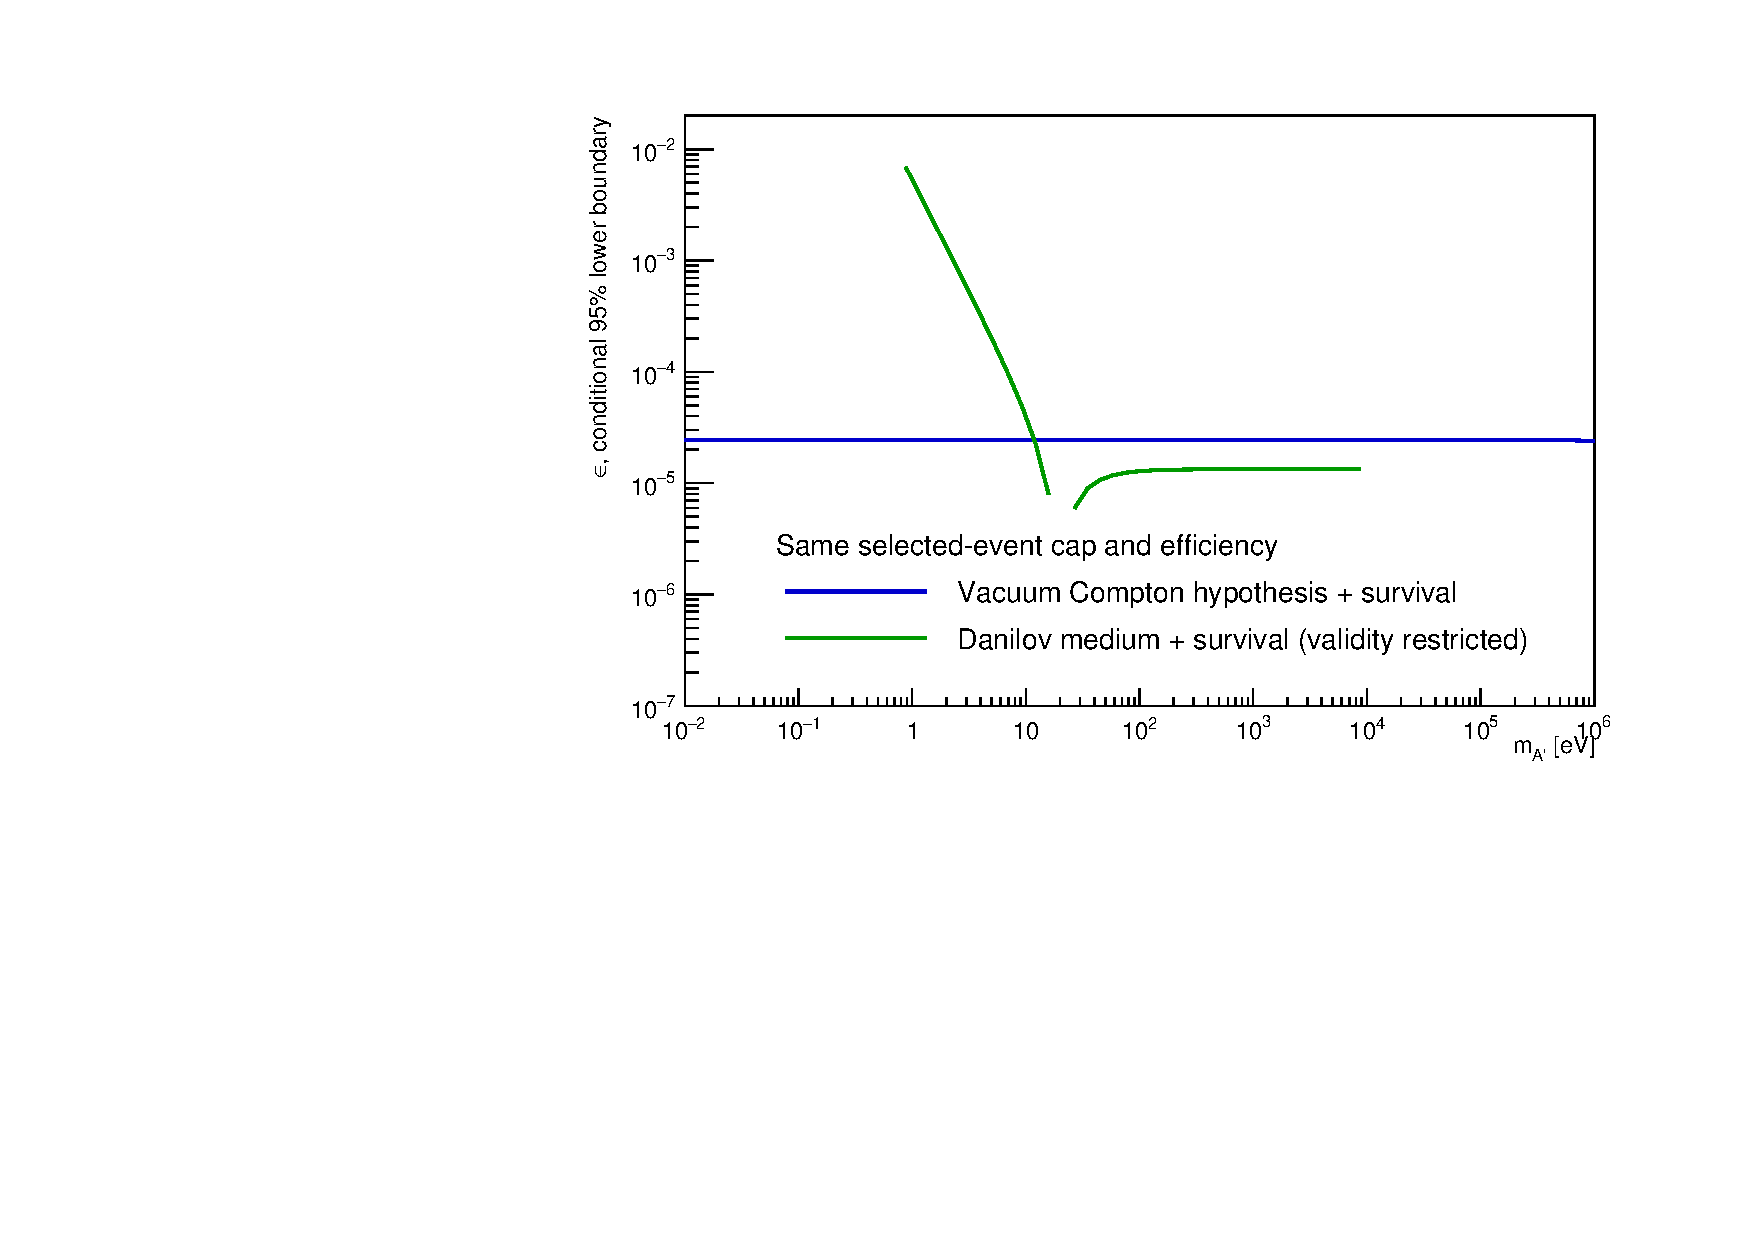
\includegraphics[width=\linewidth]{work/reactor_sensitivity/output/conditional_limits.pdf}
\caption{\both{Same selected-event cap and efficiency in both hypotheses. The vacuum curve illustrates the massive Compton model; it is not a valid low-mass material exclusion. The medium curve is restricted to its relativistic validity range and excludes the resonance window.}{Mismo límite de eventos seleccionados y eficiencia en ambas hipótesis. La curva de vacío ilustra el modelo Compton masivo; no es una exclusión material válida a masa baja. La curva en el medio está restringida a su régimen relativista y excluye la ventana resonante.}}
\end{figure}

\section{\both{Reproduction status and reuse}{Estado de reproducción y reutilización}}
\both{The only PDF in \texttt{papers\_init} is Park. Its Figure 1 is recalculated and compared with its vector paths: the heavier-mass spectra disagree, so the full figure is not reproduced. Figure 2 combines TEXONO, NEOS and external astronomical, cosmological and laboratory exclusions. We calculate the TEXONO component, which also disagrees with the printed bound. The original external data and the private NEOS background analysis are not supplied; the complete Figure 2 is not reproduced. Showing the published page or digitizing it would not change this status.}
{El único PDF en \texttt{papers\_init} es Park. Su figura 1 se recalcula y compara con sus trazos vectoriales: los espectros de mayor masa discrepan y la figura completa no está reproducida. La figura 2 combina TEXONO, NEOS y exclusiones astronómicas, cosmológicas y de laboratorio. Calculamos la componente TEXONO, que también discrepa con el límite impreso. No se aportan los datos externos originales ni el análisis privado del fondo de NEOS; la figura 2 completa no está reproducida. Mostrar la página publicada o digitalizarla no cambia ese estado.}

\both{Run \texttt{bash work/reactor\_sensitivity/run.sh} from the project root. Edit \texttt{config.conf} for power, baseline, detector mass, exposure, composition, ROI, efficiency, medium parameters and the event cap. Supply a separately justified \texttt{N95\_events} for a different likelihood, or use the documented Gaussian excess/error option. Background is represented by the excess and its uncertainty, not by a simulated spectrum. The current sub-MeV scan requires an ROI lower edge above 1 MeV. General lower-energy detectors need atomic and response modeling before reuse.}
{Ejecutar \texttt{bash work/reactor\_sensitivity/run.sh} desde la raíz. Editar \texttt{config.conf} para potencia, distancia, masa del detector, exposición, composición, ROI, eficiencia, parámetros del medio y límite de eventos. Proporcionar \texttt{N95\_events} justificado por separado para otra verosimilitud, o usar la opción gaussiana documentada de exceso/error. El fondo está representado por el exceso y su incertidumbre; no por un espectro simulado. Este barrido sub-MeV exige que la ROI comience por encima de 1 MeV. Para otros detectores de menor energía se necesita modelar ligadura atómica y respuesta.}

\both{New C++ functions implement decay propagation, cached event integration and the first upward crossing of the event cap. ROOT supplies quadrature and rendering; existing project code supplies the checked trace and source convolution. No new microscopic amplitude is claimed. The executed checks cover scaling, zero-distance and zero-mixing survival, analytic root recovery, absent roots, quadrature convergence and event-cap closure. Unchecked: the exact near-threshold loop, reactor transport, detector response, polarization transport in a Compton-produced beam, raw TEXONO likelihood and the full published exclusion compilation.}
{Las funciones nuevas en C++ implementan propagación, integración de eventos con pesos precalculados y el primer cruce ascendente del límite de eventos. ROOT aporta cuadratura y gráficos; el código previo aporta la traza verificada y la convolución de la fuente. No se afirma una amplitud microscópica nueva. Los controles ejecutados cubren escalas, supervivencia a distancia y mezcla nulas, recuperación de raíces analíticas, raíces ausentes, convergencia de cuadratura y cierre del límite de eventos. Sin verificar: lazo exacto cerca del umbral, transporte en el reactor, respuesta del detector, transporte de polarización del haz Compton, verosimilitud original de TEXONO y compilación completa de exclusiones.}
